%% USPSC-Introducao.tex

% ----------------------------------------------------------
% Introdução (exemplo de capítulo sem numeração, mas presente no Sumário)
% ----------------------------------------------------------
\chapter[Introduction]{Introduction}

During the last decade, the world has seen an increase in participation of renewable sources in power generation, leaded mainly by wind and solar energy. These green technologies provide an alternative to sources based on fossil fuel, lowering pollution levels and reducing greenhouse gas emissions. On the other hand, the power output from these sources rely on weather conditions and can't be fully controlled.

This increase is seen worldwide, as part of policies to reduce the human impact on climate and the environment. This `renewable wave' is leaded mainly by European countries, specially in the European Union (EU), United States (US) and China. In particular, EU has set in 2010 a strategy plan to reduce its greenhouse emissions by at least 20\% compared to 1990 levels and increase the share of renewable sources to at least 20\% by 2020 \cite{Europe2020}.

Brazil does not lag far behind EU regarding renewable sources policies. In 2002, the country passed a bill that, among other actions, creates the Program of Incentive to Alternative Electric Energy Sources (PROINFA). This program aims to increase the share of wind, solar, small hydro and biomass energy production. The final goal is to have these resources corresponding to 10\% of Brazil's annual energy consumption \cite{Brazil2002}.

\section{Wind Energy}

Those policies stimulated the increase of wind energy participation, reaching a scenario where it is the main energy source of some countries. In the EU, wind energy alone generated 362 TWh in 2018, covering 14\% of the electricity demand, a share 2\% higher than 2017. Breaking down to countries, Denmark leads in this sector, with 41\% of its demand supplied by wind power plants, followed by Ireland (28\%), Portugal (24\%) and Germany (21\%). The total installed capacity across the 28 EU countries is 178.8 GW, with Germany in first position, with a total installed capacity of 59.3 GW, followed by Spain and the UK, with 23.5 and 21.0 GW installed, respectively \cite{WindEurope2019}. Figure \ref{fig: EUrank} displays the detailed percentage of electricity demand covered by wind in the EU.

\begin{figure}[]
	\caption{Share of electricity demand in the EU covered by wind energy}
	\begin{center}
		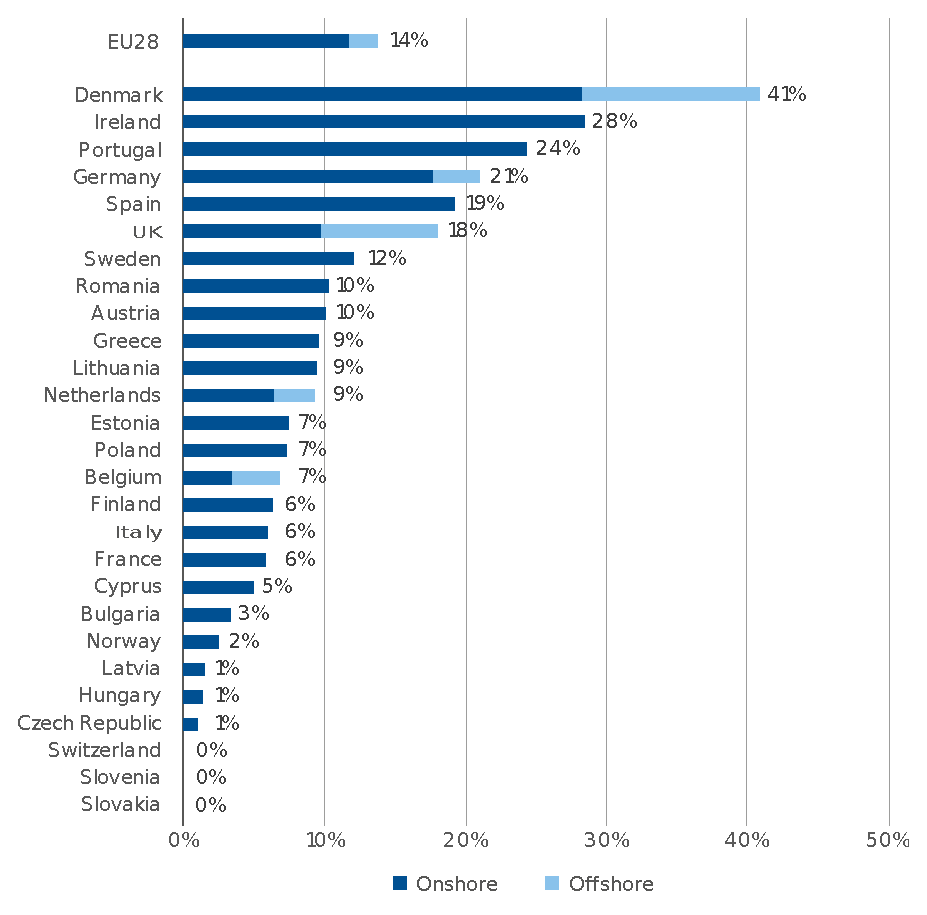
\includegraphics[scale=0.5]{Images/EUrank.eps}
	\end{center}
	\label{fig: EUrank}
	\legend{Source: Wind Europe}	
\end{figure}

In Brazil, wind energy contributed with 42.4 TWh during 2017, resulting in a participation share of 7.2\%. But, while other sources, such as hydro and coal, had its share lowered, wind energy had the highest variation among sources comparing to 2016, increasing its contribution by 26.5\% \cite{EPE2018}. In therms of installed capacity, wind power plants appear in \nth{2} place, with 14.7 GW installed, only behind hydro power plants \cite{ABEEolica2018}, as shown in Figure \ref{fig: BRshare}.

\begin{figure}[b]
	\caption{Electricity generation in Brazil by source}
	\begin{center}
		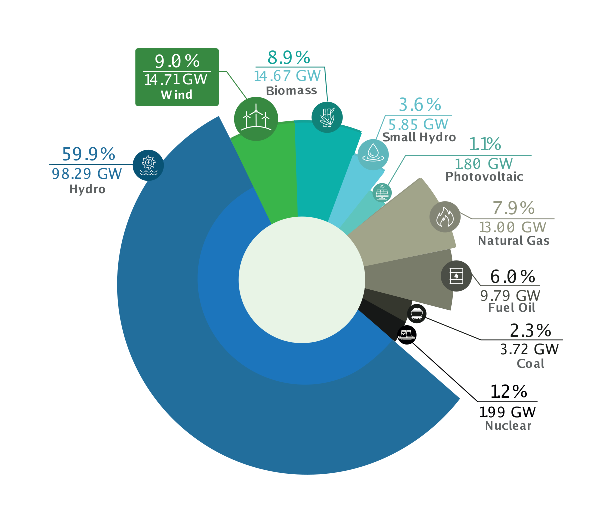
\includegraphics[scale=0.75]{Images/BRshare19.eps}
	\end{center}
	\label{fig: BRshare}
	\legend{Source: ABEE\'olica}
\end{figure}

However, there is plenty of energy yield for this source to be explored. Studies show that Brazil has potential to generate 272.2 TWh per year, with an installed capacity of 143.5 GW. The Northeast Region has the higher potential, with an annual energy yield of 144.3 TWh and potential to host up to 75.0 GW \cite{Atlas2001}. Also, the wind regime in the Northeast Region is complimentary to the water regime of the main river responsible to power generation in the region, as presented by Figure \ref{fig: WindWater}. This characteristic would help controlling reservoir water level during dry season, an important resource not only for power generation, but also irrigation of crops and water supply \cite{ANEEL2005}.

\begin{figure}
	\caption{Wind and water regime in the Northeast Region}
	\begin{center}
		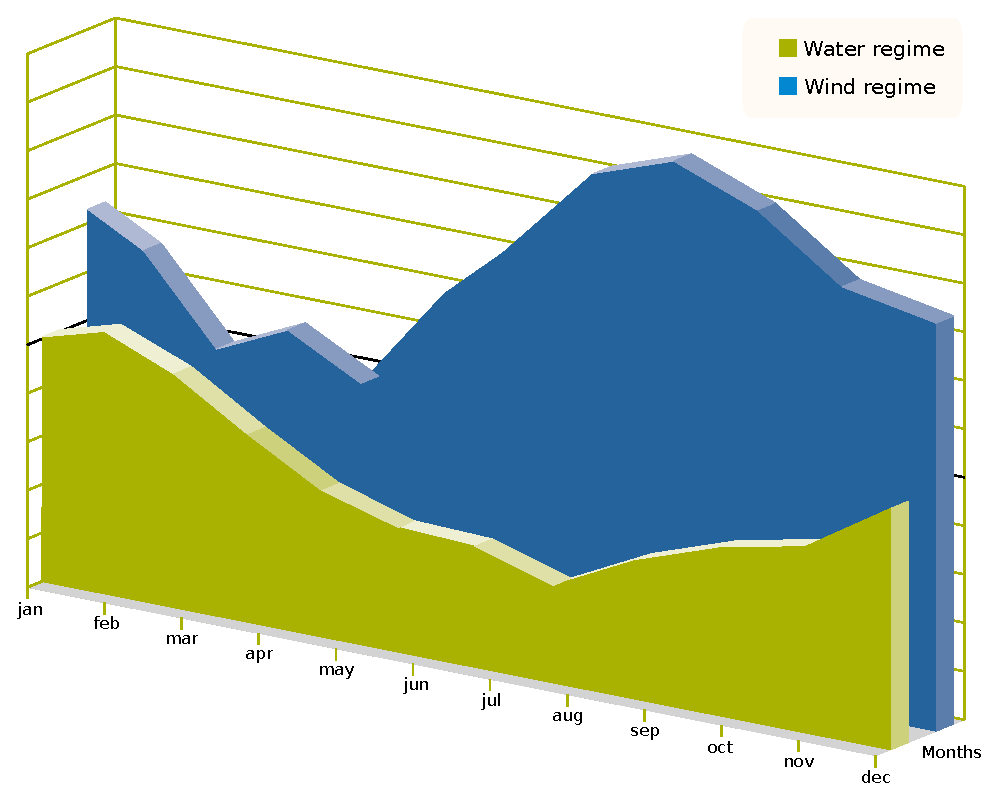
\includegraphics[scale=0.5]{Images/WindWater.eps}
	\end{center}
	\label{fig: WindWater}
	\legend{Source: ANEEL}
\end{figure}

With all this information in hand, it is only reasonable to assume that wind energy will increase its participation in electricity generation. But, in order to allow this growth, studies about how wind generators and power plants behave during faults in the grid are needed.

\section{Wind Turbine Model}

With a growing share of energy covered by wind, system operators must consider how wind turbines affect the system stability during faults and maneuvers. To do so, mathematical models capable of describing these machines' behaviour are crucial. Obtaining these models, on the other hand, is not an easy task, due to considerable amount of wind turbines in large power plants, with different manufacturers, technologies, sizes, distances from point of connection and wind conditions. Thus, a model that describes well a particular turbine in a power plant, won't necessarily work for its neighboring generators. Also, due to industrial secrecy, manufacturers provide little or no information about how their turbines behave. Furthermore, having one model for every wind turbine within a power plant would result in a mathematical problem with high complexity and computational cost \cite{Erlich2012}.

To address this problem, studies such as \cite{Muljadi2008}, \cite{Ellis2011}, \cite{council2008wecc} and \cite{Asmine2011}, motivated specially by the Institute of Electrical and Electronics Engineers (IEEE) and the Western Electricity Coordinating Council (WECC), developed generic models able to predict the behaviour of entire wind power plants. Such models reduced the problem complexity, since they were composed of a single equivalent generator. A two-machine model is needed only in rare cases, such as when the wind power plant is composed of two or more types of wind turbines \cite{Ellis2011}.

These studies have also shown that commercial wind turbine generators could be sorted into four basic types, according to its technology \cite{Ellis2011}. These types are described in the following subsections.

\subsection{Type 1 Wind Turbine}

\subsection{Type 2 Wind Turbine}

\subsection{Type 3 Wind Turbine}

\subsection{Type 4 Wind Turbine}
